\section{Referencia de la Clase linpresupuesto}
\label{classlinpresupuesto}\index{linpresupuesto@{linpresupuesto}}
Muestra y administra una l\'{\i}nea de detalle del un presupuesto.  


{\tt \#include $<$linpresupuesto.h$>$}

Diagrama de colaboraci\'{o}n para linpresupuesto:\begin{figure}[H]
\begin{center}
\leavevmode
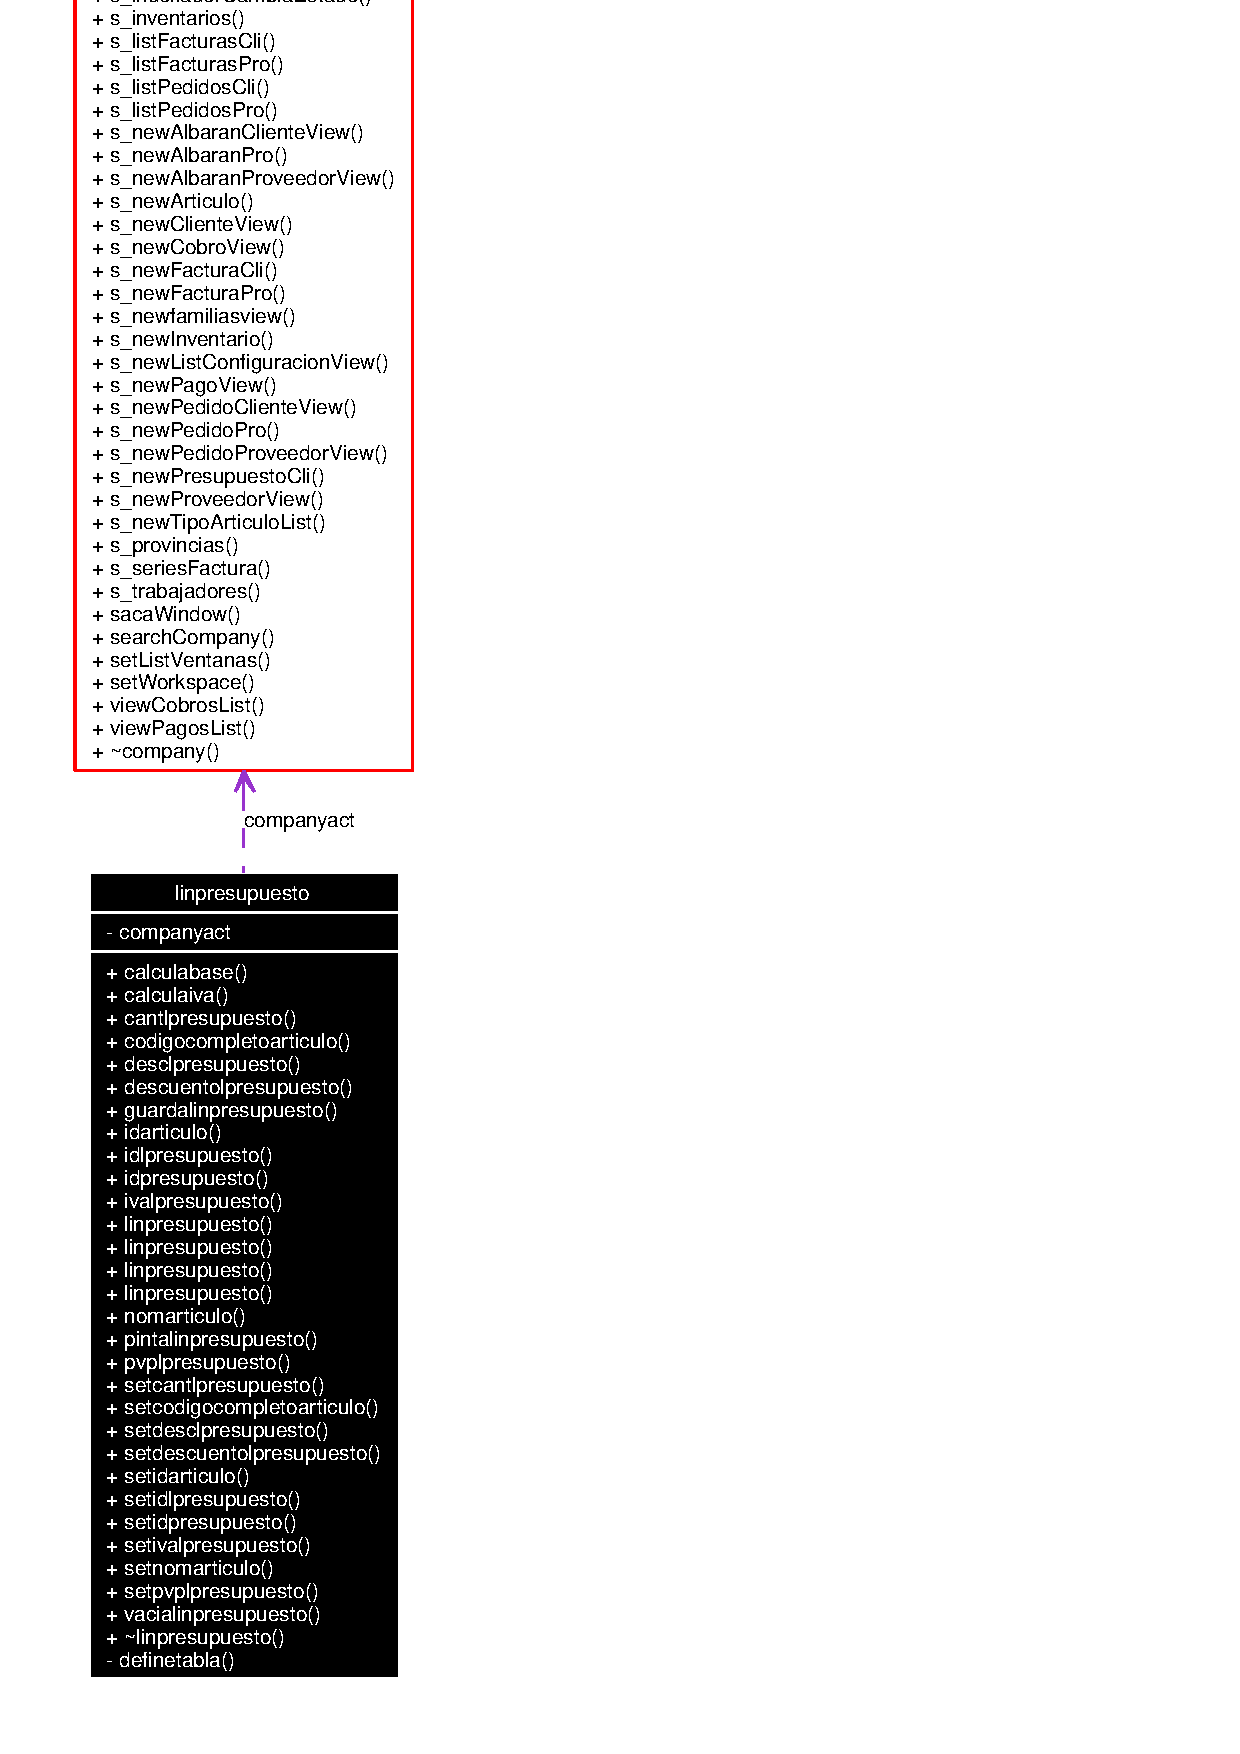
\includegraphics[width=99pt]{classlinpresupuesto__coll__graph}
\end{center}
\end{figure}
\subsection*{M\'{e}todos p\'{u}blicos}
\begin{CompactItemize}
\item 
float {\bf calculabase} ()\label{classlinpresupuesto_a0}

\begin{CompactList}\small\item\em Hace el c\'{a}lculo de la base imponible de la l\'{\i}nea. \item\end{CompactList}\item 
float {\bf calculaiva} ()\label{classlinpresupuesto_a1}

\begin{CompactList}\small\item\em Hace el c\'{a}lculo del IVA de la l\'{\i}nea. \item\end{CompactList}\item 
QString {\bf cantlpresupuesto} ()\label{classlinpresupuesto_a2}

\item 
QString {\bf codigocompletoarticulo} ()\label{classlinpresupuesto_a3}

\item 
QString {\bf desclpresupuesto} ()\label{classlinpresupuesto_a4}

\item 
QString {\bf descuentolpresupuesto} ()\label{classlinpresupuesto_a5}

\item 
void {\bf guardalinpresupuesto} ()\label{classlinpresupuesto_a6}

\item 
QString {\bf idarticulo} ()\label{classlinpresupuesto_a7}

\item 
QString {\bf idlpresupuesto} ()\label{classlinpresupuesto_a8}

\item 
QString {\bf idpresupuesto} ()\label{classlinpresupuesto_a9}

\item 
QString {\bf ivalpresupuesto} ()\label{classlinpresupuesto_a10}

\item 
{\bf linpresupuesto} ({\bf company} $\ast$, cursor2 $\ast$)\label{classlinpresupuesto_a11}

\item 
{\bf linpresupuesto} ({\bf company} $\ast$, QString, QString, QString, QString, QString, QString, QString, QString, QString, QString)
\item 
{\bf linpresupuesto} ({\bf company} $\ast$, QString)\label{classlinpresupuesto_a13}

\item 
{\bf linpresupuesto} ({\bf company} $\ast$)\label{classlinpresupuesto_a14}

\item 
QString {\bf nomarticulo} ()\label{classlinpresupuesto_a15}

\item 
virtual void {\bf pintalinpresupuesto} ()\label{classlinpresupuesto_a16}

\item 
QString {\bf pvplpresupuesto} ()\label{classlinpresupuesto_a17}

\item 
void {\bf setcantlpresupuesto} (QString val)\label{classlinpresupuesto_a18}

\item 
void {\bf setcodigocompletoarticulo} (QString)\label{classlinpresupuesto_a19}

\item 
void {\bf setdesclpresupuesto} (QString val)\label{classlinpresupuesto_a20}

\item 
void {\bf setdescuentolpresupuesto} (QString val)\label{classlinpresupuesto_a21}

\item 
void {\bf setidarticulo} (QString)
\item 
void {\bf setidlpresupuesto} (QString val)\label{classlinpresupuesto_a23}

\item 
void {\bf setidpresupuesto} (QString val)\label{classlinpresupuesto_a24}

\item 
void {\bf setivalpresupuesto} (QString val)\label{classlinpresupuesto_a25}

\item 
void {\bf setnomarticulo} (QString val)\label{classlinpresupuesto_a26}

\item 
void {\bf setpvplpresupuesto} (QString val)\label{classlinpresupuesto_a27}

\item 
void {\bf vacialinpresupuesto} ()\label{classlinpresupuesto_a28}

\end{CompactItemize}


\subsection{Descripci\'{o}n detallada}
Muestra y administra una l\'{\i}nea de detalle del un presupuesto. 



\subsection{Documentaci\'{o}n del constructor y destructor}
\index{linpresupuesto@{linpresupuesto}!linpresupuesto@{linpresupuesto}}
\index{linpresupuesto@{linpresupuesto}!linpresupuesto@{linpresupuesto}}
\subsubsection{\setlength{\rightskip}{0pt plus 5cm}linpresupuesto::linpresupuesto ({\bf company} $\ast$, QString, QString, QString, QString, QString, QString, QString, QString, QString, QString)}\label{classlinpresupuesto_a12}


La carga r\'{a}pida tiene un comportamiento poco restrictivo para aumentar la eficiencia. 

\subsection{Documentaci\'{o}n de las funciones miembro}
\index{linpresupuesto@{linpresupuesto}!setidarticulo@{setidarticulo}}
\index{setidarticulo@{setidarticulo}!linpresupuesto@{linpresupuesto}}
\subsubsection{\setlength{\rightskip}{0pt plus 5cm}void linpresupuesto::setidarticulo (QString)}\label{classlinpresupuesto_a22}


Estas funciones no est\'{a}n como debe, el uso de cada una de ellas debe hacer cambios sobre la base de datos. 

La documentaci\'{o}n para esta clase fu\'{e} generada a partir de los siguientes archivos:\begin{CompactItemize}
\item 
linpresupuesto.h\item 
linpresupuesto.cpp\end{CompactItemize}
